\chapter{深度卷积神经网络}
% TODO:深度学习在雷达信号处理中的应用扩展
\section{引言}
人工神经网络\cite{hebb2005organization}是一种通过模仿大脑神经元行为进行信息处理的数学模型,但由于其无法承受大规模的参数和训练样本并且具有泛化能力差等问题。Fukushima\cite{fukushima1982neocognitron}于1982年首次提出了卷积神经网络模型,Lecun 等人对神经网络传统算法在训练上面临的计算复杂度高等问题进行了改进,提出了基于梯度下降的优化算法\cite{lecun1998gradient}和BP算法\cite{lecun1989backpropagation}。2003年,Simard对卷积神经网络进行了简化\cite{simard2003best}。Hinton 在2006年的两篇文章\cite{hinton2006reducing,hinton2006fast}可以作为深度学习(Deep Learning,DL)正式提出的里程碑,其在工业界以及学术界掀起了巨大的浪潮,被应用于语音识别\cite{hinton2012deep}、图像识别\cite{krizhevsky2012imagenet}和自然语音处理\cite{collobert2011natural}等各种方面。 目前,其内涵已经超出了传统的多层神经网络,甚至机器学习的范畴,逐渐朝着人工智能的方向快速发展\cite{silver2017mastering}。

深度神经网络模型是一种非常强大的深度学习模型,他同时可以处理有监督和无监督学习任务。并且随着科技的发展,数据量越来越大,计算机并行能力也有了很大的提高。并且\textcolor{red}{Ciren在2011年对神经网络进行改造使其可以通过GPU进行训练计算\cite{ciresan2011flexible},并且专门针对于深度学习的芯片不断问世,例如谷歌公司的TPU\cite{jouppi2017datacenter},大大提高了深度学习的应用场景}。针对于海量数据,简单的线性模型由于无法充分利用计算能力,不再适用,可以预见在将来会有越来越多的工作应用到深度学习。

\section{基本分类}
传统上可以把深度学习分为卷积神经网络(Convolutional Neural Networks, CNN)、递归神经网络(Recurrent Neural Networks,RNN)、长短时记忆网络(Long short-term memory, LSTM)、深度信念网络(Deep Belief NetWorks,DBN)、自动编码器(AutoEncoder)、稀疏编码(Sparse Coding)、限制波尔兹曼机(Restricted Boltzmann Machine, RBM)等。

其中卷积神经网络是最流行的一种深度学习模型,通过使用卷积层极大地减少了中间层的参数数目,使学习效率更高并较少过拟合,同时卷积操作独有的局部感受野(local receptive fields)、共享权重(shared weights)和池化(pooling)三种特性也是处理序列元素分类识别的很重要的一点,权重共享策略减少了需要训练的参数,相同的权重可以让卷积核不受信号位置的影响来检测信号的特性,使得训练出来的模型泛化能力更强;池化运算可以降低网络的空间分辨率,从而消除信号的微小偏移和扭曲。

递归神经网络是一种包含循环的,允许信息持久化的神经网络模型。传统的前馈神经网络中,单独的输入完全确定了余下层的神经元的激活值。而对于递归神经网络,隐藏层和输出层的神经元的激活值不仅由当前的网络输入决定,而且包含了前面的输入的影响。长短时记忆网络是一种特殊的递归神经网络,主要用于解决递归神经网络前期模型难以训练的问题。其通过刻意设计的单元结构,在递归神经网络的基础上添加了元胞状态(cell state)用来保存长期的状态,然后通过门函数来控制此长期状态。

深度信念网络是一个概率生成模型,是由多个限制玻尔兹曼机组成,这些网络被“限制”为一个可见层和一个隐藏层,层间存在连接,但是层内的单元间不存在连接。隐藏单元被训练来捕捉在可见层表现出来的高阶数据的相关性。

通过对于以上几种最常用的深度学习方法的介绍,我们可以发现卷积神经网络是最适合处理本文这种静态类型的数据,循环或者说是不同时刻的输入对于地海杂波类型的识别并没有提高,故递归神经网络和长短时记忆网络显然不适合本问题。另一方面,深度信念网络的生成模型并不关心不同类别之间的最优分类面的位置,故其用于分类问题时,分类精度没有判别模型高。且其学习的是数据的联合分布,相比其他算法具有更高的复杂性。

\section{传统人工神经网络结构}
\textcolor{red}{深度学习在图像识别中的研究及应用——李卫}

人工神经网络是一种模拟大脑神经系统的算法,其可以从海量的训练样本中学习到一个权重函数,用来进行模式识别、分类等。神经网络主要是利用将许多个单一神经元(也称作感知器)联结在一起,一个神经元的输出就可以是另一个神经元的输入,形成一个有向无环的网络结构。首先介绍一个神经元的结构,如图\ref{fig:neural}。其神经元具有多个输入$x_1,x_2,\dots $ ,这些输入可以取0和1中的任意值。神经元对于每一个输入有权重$w_1,w_2,\dots $ 和一个总的偏置$b_0$ ,其输出为一个$\sigma(w\cdot x + b)$ ,这里的 $\sigma$为该神经元的激活函数,定义为:
\begin{equation}
  \sigma(z)\equiv\frac{1}{1+e^{-z}}  
\end{equation}
,此处的激活函数称作S型激活函数,常使用的还有$ReLU $ 等激活函数。
\begin{figure}
  \centering
  \includestandalone[width=\textwidth]{figures/neural}
  \caption{神经元}
  \label{fig:neural}  
\end{figure}

多个神经元分层互联可以形成神经网络。图\ref{fig:network}是一个简单的神经网络,其中圆圈表示神经网络的输入,标上$ +1$的圆圈被称为偏置节点,也就是截距项。神经网络最左边的一层叫做输入层,最右的一层叫做输出层(本例中,输出层只有一个节点)。中间所有节点组成的一层叫做隐藏层(不能在训练样本集中观测到它们的值)。同时可以看到,以上神经网络的例子中有3个输入单元(偏置单元不计在内),3个隐藏单元及一个输出单元。

\begin{figure}
  \centering
  \includestandalone[width=\textwidth]{figures/network1}
  \caption{神经网络}
  \label{fig:network}  
\end{figure}

本例中网络的层数为 $ n_l=3$ ,将第 $ l $层记为 $ L_l$ ,于是$  L_1$ 是输入层,输出层是 $ L_{n_l} $。本例神经网络有参数 $ (W,b) = (W^{(1)}, b^{(1)}, W^{(2)}, b^{(2)}) $,其中 $ W^{(l)}_{ij}$ (下面的式子中用到)是第 $ l $层第 $ j$ 单元与第 $ l+1 $层第$  i$ 单元之间的联接参数(其实就是连接线上的权重,注意标号顺序),$ b^{(l)}_i $是第$  l+1 $层第$  i$ 单元的偏置项。因此在本例中, $ W^{(1)} \in \Re^{3\times 3}$ , $ W^{(2)} \in \Re^{1\times 3}$ 。注意,没有其他单元连向偏置单元(即偏置单元没有输入),因为它们总是输出 $ +1$。同时,我们用 $ s_l $表示第$  l$ 层的节点数(偏置单元不计在内)。

$ a^{(l)}_i$ 表示第$  l $层第 $ i$ 单元的激活值(输出值)。当$  l=1$ 时,$  a^{(1)}_i = x_i $,也就是第$  i $个输入值(输入值的第 $ i$ 个特征)。对于给定参数集合$  W,b $,我们的神经网络就可以按照函数 $ h_{W,b}(x)$ 来计算输出结果。本例神经网络的计算步骤如下:
\begin{align}
a_1^{(2)} &= f(W_{11}^{(1)}x_1 + W_{12}^{(1)} x_2 + W_{13}^{(1)} x_3 + b_1^{(1)})  \\
a_2^{(2)} &= f(W_{21}^{(1)}x_1 + W_{22}^{(1)} x_2 + W_{23}^{(1)} x_3 + b_2^{(1)})  \\
a_3^{(2)} &= f(W_{31}^{(1)}x_1 + W_{32}^{(1)} x_2 + W_{33}^{(1)} x_3 + b_3^{(1)})  \\
h_{W,b}(x) &= a_1^{(3)} =  f(W_{11}^{(2)}a_1^{(2)} + W_{12}^{(2)} a_2^{(2)} + W_{13}^{(2)} a_3^{(2)} + b_1^{(2)}) 
\end{align}
 $ z^{(l)}_i $表示第$ l $层第$  i$单元输入加权和(包括偏置单元),比如,$  z_i^{(2)} = \sum_{j=1}^n W^{(1)}_{ij} x_j + b^{(1)}_i$ ,则$  a^{(l)}_i = f(z^{(l)}_i) $。

这样就可以得到一种更简洁的表示法。这里激活函数 $ f(\cdot)$ 扩展为用向量(分量的形式)来表示,即$  f([z_1, z_2, z_3]) = [f(z_1), f(z_2), f(z_3)]$ ,那么,上面的等式可以更简洁地表示为:

\begin{align}
z^{(2)} &= W^{(1)} x + b^{(1)} \\
a^{(2)} &= f(z^{(2)}) \\
z^{(3)} &= W^{(2)} a^{(2)} + b^{(2)} \\
h_{W,b}(x) &= a^{(3)} = f(z^{(3)})
\end{align}

将上面的计算步骤叫作前向传播。用$  a^{(1)} = x$ 表示输入层的激活值,那么给定第$  l$ 层的激活值 $ a^{(l)}$ 后,第 $ l+1$ 层的激活值 $ a^{(l+1)}$ 就可以按照下面步骤计算得到:

 \begin{align}
z^{(l+1)} &= W^{(l)} a^{(l)} + b^{(l)}   \\
a^{(l+1)} &= f(z^{(l+1)})
\end{align}

将参数矩阵化,使用矩阵-向量运算方式,我们就可以利用线性代数的优势对神经网络进行快速求解。

也可以构建另一种结构的神经网络(这里结构指的是神经元之间的联接模式),也就是包含多个隐藏层的神经网络。最常见的一个例子是 $  n_l$ 层的神经网络,第$   1 $层是输入层,第$   n_l$ 层是输出层,中间的每个层 $  l$ 与层 $  l+1$ 紧密相联。这种模式下,要计算神经网络的输出结果,我们可以按照之前描述的等式,按部就班,进行前向传播,逐一计算第 $  L_2 $层的所有激活值,然后是第$  L_3$ 层的激活值,以此类推,直到第 $  L_{n_l}$ 层。这是一个前馈神经网络的例子,因为这种联接图没有闭环或回路。

神经网络也可以有多个输出单元。比如,图\ref{fig:network2}的神经网络有两层隐藏层:$  L_2 $及 $ L_3$ ,输出层$  L_4 $有两个输出单元。

\begin{figure}
  \centering
  \includestandalone[width=\textwidth]{figures/network2}
  \caption{具有多个输出单元的神经网络示意图}
  \label{fig:network2}  
\end{figure}

要求解这样的神经网络,需要样本集  $ (x^{(i)}, y^{(i)})$ ,其中 $ y^{(i)} \in \Re^2$ 。
\section{深度卷积神经网络}
\textcolor{red}{深度卷积神经网络在车牌和人脸检测领域的应用研究-张勇 test}

在分类器设计方面,本章设计利用卷积神经网络的分类器。典型的卷积神经网络由深层结构堆叠在一起的多个不同的层组成:输入层,多组卷积和池化层,有限数量的完全连接的隐藏层,以及输出层。其中最主要的部分为卷积层。其利用输入数据中的局部结构,将整个输入空间划分成很小的隐藏单元。将各个隐藏单元的权重构建得到的卷积核作用于整个输入空间,从而得到特征向量。利用这种机制,我们不仅大大减少了参数数量同时提高了数据的平移不变性。
  
其基本架构如图\ref{fig:network}所示,最左边的为输入层,其中的神经元为输入神经元。最右边的输出层包含有输出神经元,可以有一个也可以由多个。中间层为隐藏层,这部分为需要进行主要设计,也是各种神经网络模型的主要区别之处。为了增强其泛化能力,一般情况下有扩增路径(将多个分支包含在架构中)、金字塔形状(在整个架构中应该有一次整体的平滑的下采样,而且该下采样应该与信道数量的增长结合起来)、规范层输入(使层输入标准化,使所有输入样本更加平等)等各种设计法则,此部分需要根据实际问题以及测试结果不断调整。

\subsection{卷积}
深度卷积神经网络在特征提取过程中一个主要操作为卷积,在前向计算过程中,对于输入的一定区域的数据$x$和滤波器(或者说权重)$w$ 点乘后得到新的特征向量,然后滑过一个个滤波器,组成新的输出数据$s(t)=\sum_{a=-\infty}^{\infty}x(a)w(t-a) $。每个滤波器只关心数据的部分特征,当出现它学习到的特征的时候,就会呈现激活态。

深度卷积神经网络在特征提取过程中一个主要操作为卷积,在前向计算过程中,对于输入的一定区域的数据 和滤波器(或者说权重) 点乘后得到新的特征向量,然后滑过一个个滤波器,组成新的输出数据 。每个滤波器只关心数据的部分特征,当出现它学习到的特征的时候,就会呈现激活态。

\subsection{局部感受野}
对于传统的神经网络,每个输入元素会连接到每个隐藏神经元。相反,我们只是把输入的频谱数据进行小的、局部区域的连接,也即第一个隐藏层中的每个神经元会连接到一个输入神经元的一个区域。这个输入向量的区域被称为隐藏神经元的局部感受野。它是输入向量上的一个小窗口,对于每个连接学习一个权重而隐藏神经元同时也学习一个总的偏置。通过在整个输入频谱数据上交叉移动局部感受野,可以构建起第一个隐藏层。

\subsection{共享权重和偏置}
上面已经说过对于每个隐藏神经元具有一个偏置和连接到它的局部感受野的权重,同时对于该层的所有的隐藏神经元中每一个使用相同的权重和偏置。也即,对第$j$个隐藏神经元,输出为:
$\sigma(b+\sum_{m=1}^M w_m a_{j+m}) $
这里$\sigma$是神经元的激活函数,$b$是偏置的共享值,$w_m$是一个共享权重的$1\times M$向量,$a_k$表示位置$k$的输入激活值。这意味着第一个隐藏层的所有神经元检测完全相同的特征,只是在输入频谱数据的不同位置,因此卷积网络可以很好地适应频谱数据的布拉格峰偏移情况。

\subsection{池化}
我们在通过卷积获得了特征之后,下一步我们希望利用这些特征去做分类。理论上讲,人们可以用所有提取得到的特征去训练分类器,例如$softmax$分类器(多分类的逻辑回归分类器),但这样做面临着计算量的挑战,除此以外过多的特征向量,也容易导致过拟合。

深度卷积神经结构具有过拟合的自然趋势,虽然可以通过权重共享来减少参数的数量。但是由于大多数情况下,估计集的数量比训练集大一个数量级,使得神经网络模型的泛化能力不足。在每个训练迭代中,每个隐藏单元以预定概率被随机删除,删除后学习过程继续。这些被称作$dropout$的随机扰动有效地防止了神经网络学习过程的依赖关系,并在隐藏的单元之间创建了复杂的关系。这样增加了网络模型的复杂度,从而提高深度神经网络模型的泛化能力。
\subsection{激活函数}
激活函数的选择是构建卷积神经网络模型的一个非常重要的方面。正如前一节所述,传统的神经网络模型中通常选择Sigmod或双曲正切作为激活函数。\textcolor{red}{介绍ReLU的优越性,同时修改公式表示方法}。然而,我们通常在卷积神经网络中使用以下ReLU激活函数。
\begin{equation}
F(x) = max (0, x)
\end{equation}
ReLU具有优于传统激活函数的几个优点:更快的计算速度和更有效的梯度传播(它们不像S形单元那样饱和),生物学可能性和稀疏激活结构。尽管它们结构简单,但仍然保持足够的辨别性质。其缺点之一是随机权重的初始状态,多个单位可能过早地落入死区(零输出的恒定梯度)。因此,当与整个连接层进行全连接时,Sigmod激活函数的效果更好。
\begin{equation}
F(x) = \frac{1}{1-exp(x)}
\end{equation}
\subsection{网络的训练与学习}
\textcolor{red}{添加文字描述,关于梯度下降算法。}

如果用符号$x $表示一个训练输入,用$y=y(x) $ 表示对应的期望输出。学习算法的主要目的是找到一个权重$w$和偏置$b$使得网络的输出$y(x) $ 可以拟合所有的训练输入$x$ 。为此可以定义一个损失函数(又称作代价函数):
\begin{equation}
  C(w,b)\equiv \frac{1}{2n}\sum_x||y(x)-a||^2 
\end{equation}
这里$w$表示所有的网中权重的集合,$b$ 是所有的偏置, $n$是训练输入数据的个数,$a$ 是表示当输入为$x$ 时输出的向量,求和总是在总的训练输入$x$ 上进行的。上述损失函数为均方误差,其是可以根据不同的问题进行不同的设置的。从定义可以看出, $C(w,b) $越小说明分类越准确,那么训练神经网络的目的就是找到最小化二次代价函数 $C(w,b) $的权重和偏置。
\begin{figure}
	\centering
	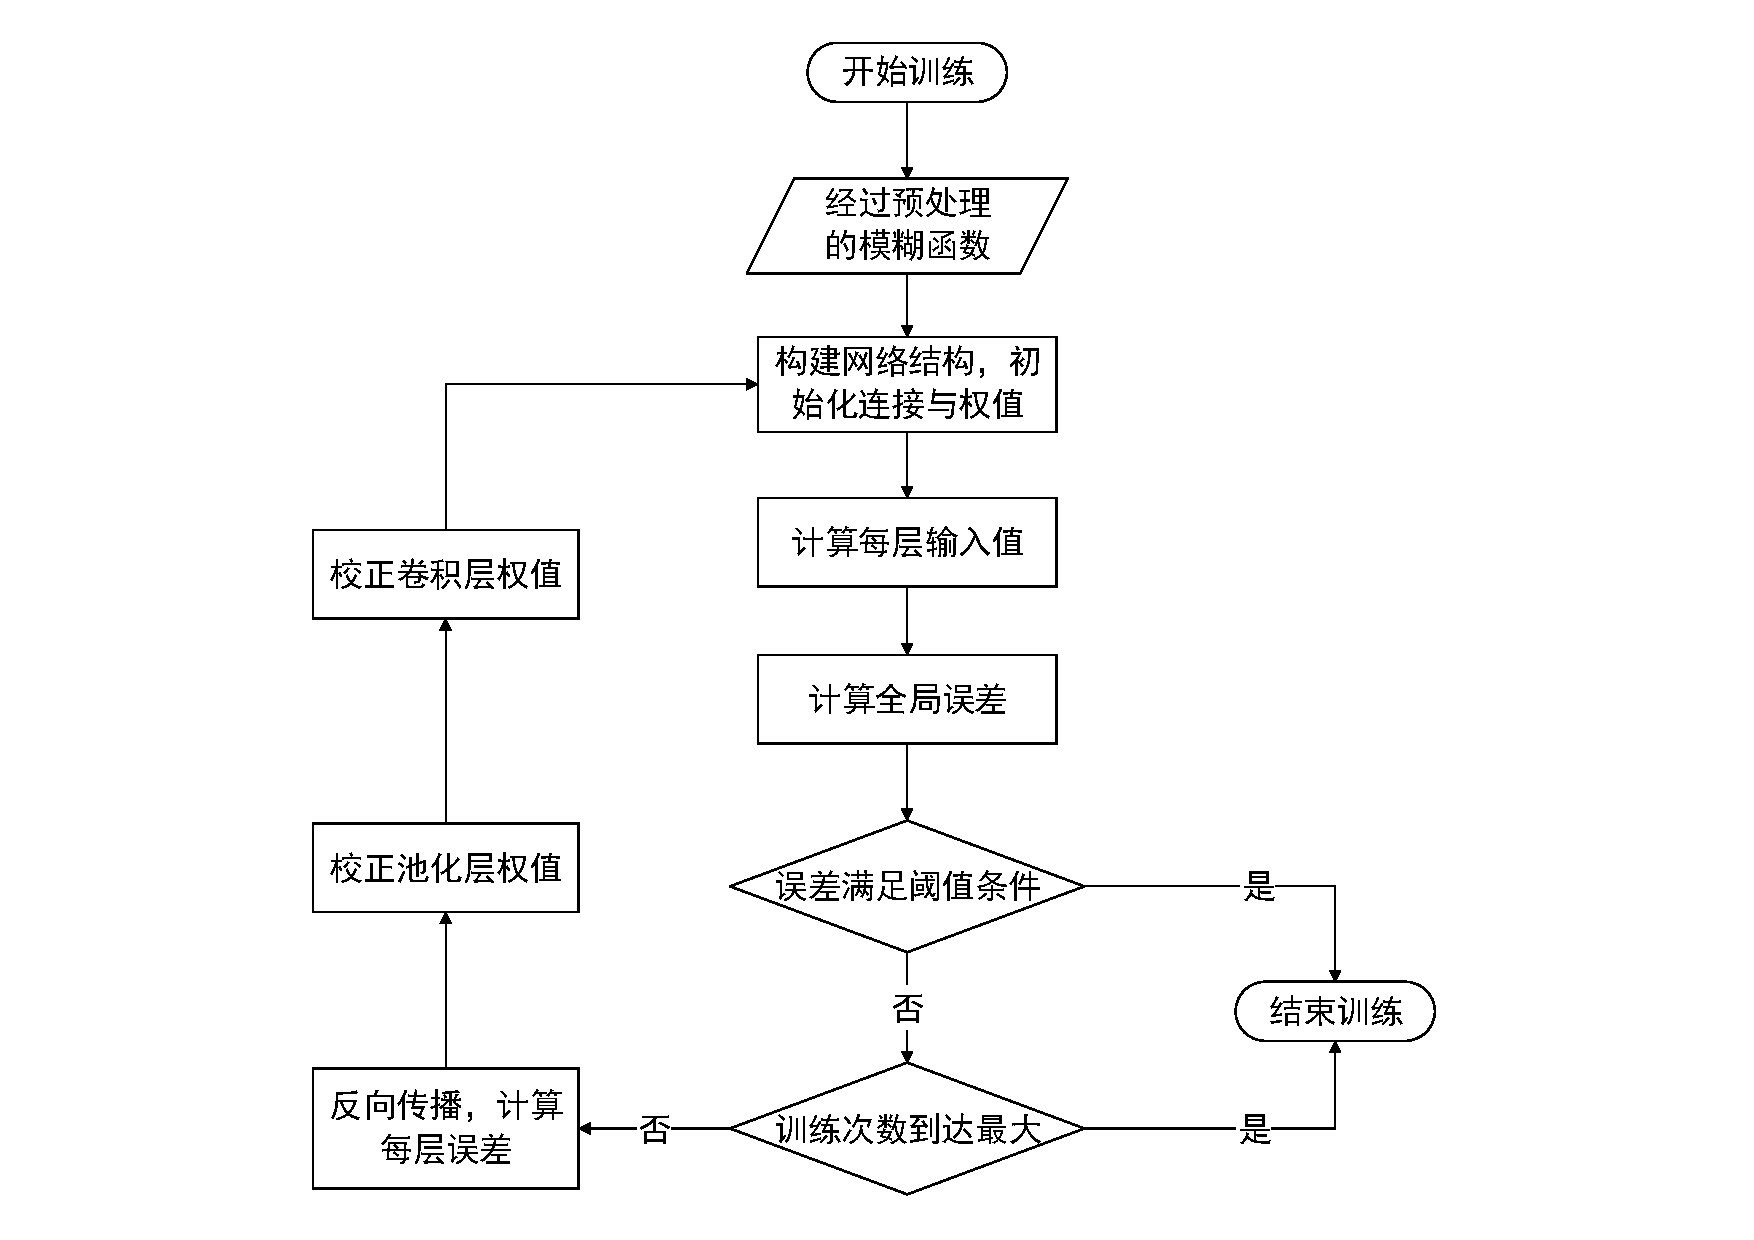
\includegraphics[width=\textwidth]{figures/cnn_flow.pdf}
	\caption{深度卷积神经网络算法训练流程图}
\end{figure}
将上述问题一般化也就是,最小化任意的具有 $m $个变量的多元实值函数 $C(v) $, $v=v_1,v_2,\dots,v_m $。对于这种具有大量变量的函数的解析解是极其复杂的,其比较合理的思路为利用数值计算的方法求取其极值点。每次对于$C $ 中的自变量 添加一个微小的变化$\Delta v $ ,根据此变化反映出来的$C $ 的变换 $\Delta C $更新下次的微小变化,从而使得$C $ 可以持续减小。对$C $ 中自变量的变化$\Delta v=(\Delta v_1,\dots,\Delta v_m)^T $ , $\Delta C $将会变为
\begin{equation}
    \Delta C \approx \bigtriangledown C \cdot \Delta v   
\end{equation}
,这里的梯度$\bigtriangledown C $ 定义如下:
\begin{equation}
\bigtriangledown C \equiv (\frac{\partial C}{\partial v_1},\dots,\frac{\partial C}{\partial v_m})^T 
\end{equation}
其把$v$的变化关联为$C$的变化,假设我们选取
$\Delta v=-\eta \bigtriangledown C $
这里的$\eta $是学习率,一般取一个很小的正数,这时候有
\begin{equation}
\Delta C \approx -\eta\bigtriangledown C\cdot\bigtriangledown C=-\eta||\bigtriangledown C||^2 \leq 0  
\end{equation}
也即如果利用更新规则
$v \rightarrow v'=v-\eta \bigtriangledown C$,
$C $会持续减小,此更新规则即为梯度下降算法,这就是最基本的学习算法。可以根据选择不同的代价函数 $C $或者通过计算来完成学习速率的选择等各种技术对学习算法进行优化。

\section{深度卷积神经网络在雷达信号处理中的应用}
% \textcolor{red}{SAR 雷达图像处理 基于深度学习的多摄像机协作监控系统}

由于深度卷积网络在图像处理等领域的卓越表现,一部分学者也开始将其应用于雷达的信号处理领域。在早前,大部分应用均集中于合成孔径雷达(Synthetic aperture radar,SAR)图像处理,主要用于遥感中的地物分类领域\cite{chen2014sar,xie2014multilayer,lv2014classification}。Xie \cite{xie2014multilayer}基于深度学习提出了一种自动学习极化合成孔径雷达(PolSAR)中多层特征的方法。文中主要利用了叠加稀疏自编码器(SAE),使用少量标签微调他们的方法的参数。最终,实验结果证实了其所提出的方法在分类精度和视觉效果方面具有显著的提升。

而随着深度学习技术的发展,一部分学者逐渐把深度学习引入新的领域。恒虚警 (Constant False Alarm Rate, CFAR)检测是雷达系统常用的目标检测算法,传统的方法可以分为几种在不同环境下具有不同性能的方法。Rohman \cite{rohman2017classification}提出了一种隐含神经元数变化的集成神经网络分类器,对雷达环境进行分类的自适应CFAR检测方法。在多目标和杂波边界环境下,该方法仍然能够表现出最好的性能。Kim提出了一种基于多普勒雷达的深度卷积神经网络(DCNNs)用于人体检测和活动分类的方法\cite{kim2016human}。 他们主要针对传统解决方案中依赖于手工特征的设计这个问题,提出了将DCNN直接应用于人体检测和活动分类问题的原始多普勒频谱图。DCNN可以使用测量数据共同学习必要的特征和分类边界,而不需要在多普勒信号上使用任何明确的特征,并且取得了很高的精度。Zhang \cite{zhang2017novel}针对不同运动形式和复杂杂波背景下的多目标跟踪问题,通过将传统的MN逻辑航迹起始算法与深度学习进行结合实现了在复杂杂波环境下的多目标航迹起始算法。仿真实验表明,其方法比传统的用于航迹起始的改进Hough变换要好得多,特别是在目标机动的情况下,同时该方法具有很强的鲁棒性和适应性,能够对来自不同雷达的数据进行起始。虽然应用场景逐渐增大,但是大部分的实施步骤仍然是利用二维的卷积神经网络对图像进行分类识别等,我们在此通过对雷达信号序列的分析,利用深度学习方法对一维序列雷达信号进行处理。

\section{小结}
本章总结了基本的深度学习基础。首先是其基本分类,然后针对于本文利用的深度卷积神经网络,首先介绍了传统的神经元的结构和卷积神经网络基于此的改进。在最后讨论了深度卷积神经网络在雷达信号处理中的应用。
% \begin{table}
%  \caption{测试表格}
%  \centering
%  \begin{tabular}{cccccc}
%    \toprule
%    & $h$ & $L^2$ error & Order & $L^{(\alpha,\beta)}$ error & Order \\
%    \midrule
%    \multirow{5}{4em}{$\alpha=0.85$\\ $\beta = 0.85$}
%    & 1/4   & 3.8571e-04 &      - & 3.0781e-03 &      -\\
%    & 1/8   & 1.3035e-04 & 1.5651 & 1.2640e-03 & 1.2840\\
%    & 1/16  & 3.8665e-05 & 1.7533 & 5.2782e-04 & 1.2599\\
%    & 1/48  & 4.9386e-06 & 1.8731 & 1.5519e-04 & 1.1142\\
%    \bottomrule
%  \end{tabular}
% \end{table}

